%%% packages %%%
%%%%%%%%%%%%%%%%%%%%%%%%%%%%%%%%%%%%%%%%%%%%%%%%%%%%%%%%%%%%%%%%%%%%%%%%%%%%%%%  
\documentclass[frenchb]{report}
%\usepackage{natbib}
\usepackage{hyperref}
\usepackage[toc,page]{appendix}
\usepackage[dvipsnames]{xcolor}
\usepackage[french]{babel}
\usepackage{url}
\usepackage[utf8x]{inputenc}
\usepackage{graphicx}
\graphicspath{{images/}}
\usepackage{parskip}
\usepackage{fancyhdr}
\usepackage{fancyvrb}
\usepackage{vmargin}
\usepackage{xcolor}
\usepackage{bbm}
\usepackage{amsmath,amssymb}
\usepackage{amsthm}
\usepackage{dsfont}
\usepackage{stmaryrd}
\usepackage{systeme}
\usepackage{enumitem}
\usepackage{xcolor}
\usepackage{pifont}
\usepackage{textcomp}
\usepackage{calrsfs}
\usepackage[T1]{fontenc}
\usepackage[toc,page]{appendix}
\usepackage{lipsum}
\usepackage{verbatim}
\usepackage{listings}
\usepackage{adforn}
\usepackage{float}
\usepackage{subfig}
\RequirePackage{listings}% Pour incorporer du code dans un langage de programmation

%%%  MARGE   %%%%%%%%%%%%%%%%%%%%%%%%%%%%%%%%%%%%%%%%%%%%%%%%%%%%%%%%%%%%

\setlength{\hoffset}{-18pt}        
\setlength{\oddsidemargin}{0pt} % Marge gauche sur pages impaires
\setlength{\evensidemargin}{9pt} % Marge gauche sur pages paires
\setlength{\marginparwidth}{54pt} % Largeur de note dans la marge
\setlength{\textwidth}{481pt} % Largeur de la zone de texte (17cm)
\setlength{\voffset}{-18pt} % Bon pour DOS
\setlength{\marginparsep}{7pt} % Séparation de la marge
\setlength{\topmargin}{-25pt} % Pas de marge en haut
\setlength{\headheight}{0pt} % Haut de page
\setlength{\headsep}{10pt} % Entre le haut de page et le texte
\setlength{\footskip}{27pt} % Bas de page + séparation
\setlength{\textheight}{720pt} % Hauteur de la zone de texte (25cm)

%%%%%%%%%%%%%%%%%%%%%%%%%%%%%%%%%%%%%%%%%%%%%%%%%%%%%%%%%%%%

\makeatletter
\let\thetitle\@title
\let\theauthor\@author
\let\thedate\@date
\makeatother

%%% commandes mise en page %%%
%%%%%%%%%%%%%%%%%%%%%%%%%%%%%%%%%%%%%%%%%%%%%%%%%%%%%%%%%%%%%%%%%%%%%%%%%%%%%%%        
\newcommand{\ld}{\log_{2}}
\newcommand{\R}{\mathbbm{R}}
\newcommand{\N}{\mathbbm{N}}
\newcommand{\1}{\mathbbm{1}}
\newcommand{\E}{\mathbbm{E}}
\newcommand{\V}{\mathbbm{V}}
\newcommand{\prob}{\mathbbm{P}}
\newcommand{\Nc}{\mathcal{N}}
\newcommand{\Cc}{\mathcal{C}}
\newcommand{\K}{\mathcal{K}}
\newcommand{\Xti}{\widetilde{X_i}}
\newcommand{\Xtj}{\widetilde{X_j}}
\newcommand{\Xn}{\overline{X_n}}
\newcommand{\gn}{\hat{g_n}}
\newcommand{\n}{\mathcal{N}}
\newcommand{\lv}{\mathcal{L}}
\newcommand{\thetat}{\tilde{\theta}}

\newcommand{\console}[1]{\colorbox{black}{\begin{minipage}[c]{1\linewidth}\textcolor{white}{\texttt{#1}}\end{minipage}}}

\newtheorem{prop}{Proposition}
\newtheorem{thm}{Théorème}
\newtheorem{cor}{Corollaire}
\newtheorem{lem}{Lemme}
\newtheorem{hyp}{Hypothèse}
\theoremstyle{definition}\newtheorem{defn}{Définition}
\theoremstyle{definition}\newtheorem{exm}{Exemple}
\theoremstyle{definition}\newtheorem{nota}{Notation}
\theoremstyle{definition}\newtheorem{rem}{Remarque}

\renewcommand{\qedsymbol}{\adfhangingflatleafright}

% pour incorporer le code dans le rapport
\lstdefinelanguage{Python}%
{morekeywords={import,function,for,in,if,elseif,else,true,false,end,%
		return,while,as,len,enumerate,print,range,%
		edges,src,dst,has_edge,isempty,size,zeros,minimum,},%
	sensitive=true,%
	morecomment=[n]{\#},%
	morestring=[s]{"}{"},%
	morestring=[m]{'}{'},%
}[keywords,comments,strings]%

\lstset{%
	language         = Python,
	basicstyle       = \ttfamily,
	keywordstyle     = \bfseries\color{blue},
	stringstyle      = \color{magenta},
	commentstyle     = \color{green},
	showstringspaces = false,
}

\begin{document}
%%% Pour l'annexe
\def\appendixpage{\vspace*{8cm}
\begin{center}
\Huge\textbf{Annexes}
\end{center}
}
\def\appendixname{Annexe}%

\begin{titlepage}
\begin{center}

\includegraphics[scale=0.6]{logo.png}
\hfill

\includegraphics[scale=0.35]{fds_logo.png}
\hfill

\includegraphics[scale=0.30]{images/ssd.png}\\[3cm]
\linespread{1.2}\huge {\bfseries Apprentissage Statistique }\\[0.5cm]
\linespread{1.2}\LARGE {\bfseries Détection de structures communautaires dans des réseaux}\\[1.5cm]
\linespread{1}

{\large Rédigé par\\}
{\Large \textsc{pralon} Nicolas}\\
{\Large \textsc{côme} Olivier}\\
{\Large \textsc{sene} Assane}\\[1cm]


\includegraphics[scale=0.7]{imag_logo.png}

\end{center}
\end{titlepage}
%%%%%%%%%%%%%%%%%%%%%%%%%%%%%%%%%%%%%%%%%%%%%%%%%%%%%%%%%%%%%%%%%%%%%%%%%%%%%%%%%%%%%%%%%
\tableofcontents
\newpage
%%%%%%%%%%%%%%%%%%%%%%%%%%%%%%%%%%%%%%%%%%%%%%%%%%%%%%%%%%%%%%%%%%%%%%%%%%%%%%%%%%%%%%%%%

\chapter*{Introduction}
\addcontentsline{toc}{part}{Introduction}

De multiples réseaux, y compris les réseaux sociaux, les réseaux informatiques, se divisent plus ou moins naturellement en communautés. La détection de cette structure sous-jacente aux réseaux constitue un problème actuel, et de nombreuses approches ont été développées pour y répondre. 

Dans ce rapport nous allons présenter une approche communément utilisée en apprentissage non supervisé, permettant de mesurer la validité d'un partitionnement du réseau, les défaillances de cette approche et la mise en pratique des méthodes utilisées pour y répondre. 

\section*{Concept de Modularité}
\addcontentsline{toc}{part}{Concept de Modularité}
L'étude d'éventuelles structures communautaires dans des réseaux peut formellement être présentée par l'étude de graphe. Ainsi nous considérons un réseau comme un graphe, et émettons certaines hypothèses à notre étude : 

\begin{center}
$Soit~G = (V,E)\text{, un graphe tels que }$
\end{center}
$V = \{v_1, \cdots, v_p\} \text{ l'ensemble des nœuds }$\newline
$E \subset{\{ (v_i,v_j)_{i,j \in \{1,\cdots,p\}}| i \neq j \}} = V\times V \text{ l'ensemble des arêtes du graphe}$\

G est un graphe simple, non orienté, non pondéré, non labélisé.\\

Avant de décrire l'idée mise en œuvre pour la détection de communautés, donnons quelques définitions.\\

\begin{defn}[Densité]
On appel densité d'un graphe la valeur 
\begin{center}
$D_G = \frac{|E|}{\frac{p^2-p}{2}} $
\end{center}
\end{defn}

La densité d'un graphe correspond à la fréquence d'arêtes dans le graphe, il rend compte de la connexion entre les nœuds.

\begin{defn}[Degré]
On appel degré d'un nœud $i$ la valeur 
\begin{center}
$d_i = |\{(v_i,v_j) \in E | j \in {\{1,\cdots,p\}} \}| $
\end{center}
\end{defn}
et correspond au nombre de voisin du noeud $i$.\\

\begin{defn}[Modèle nul]
On appelle modèle nul d'un graph $G$, le graph $G^*$ dont les $|E| = m$ arêtes ont été distribuées aléatoirement entre les nœuds de $G$
\end{defn}
Le modèle nul joue un modèle de référence pour lequel il n'existe aucune structure communautaire dans le réseau.\\

Revenons sur la question de détection de communautés et abordons la par étape.\\
Soit $G$ un graphe.\\
Par simplicité nous souhaitons déterminer s'il existe une division du graphe $G$ en deux communautés. Une approche intuitive est de chercher deux groupes de nœuds pour lesquels on cherche à maximiser le nombre d'arêtes entre les nœuds du groupe et à minimiser le nombre d'arêtes entre nœuds de groupes différents. 

Cependant le simple comptage des arêtes n'est pas un bon moyen de quantifier le concept de structure communautaire. Si l'on choisissait pour groupe le graphe et pour second groupe un ensemble vide, ce partitionnement serait alors optimal, mais ne répond pas au problème.

Le concept de modularité que nous allons présenter est l'idée sous laquelle, si il existait éventuellement une structure dans un graphe, alors en le comparant à son modèle nul pour lequel il n'existe aucune structure sous-jacente, nous devrions raisonnablement observer une différence entre les deux modèles.\\

\begin{defn}[Modularité]
Soit $(C_1,\cdots,C_K)$ une partition de $V$\\
On définit la modularité $Q$ de la partition comme 
\begin{center}
$Q(C_1,\cdots,C_K) = \frac{1}{2m}\displaystyle\sum_{k=1}^K \displaystyle\sum_{(v_i,v_j)\in C_k} (\1_{v_i,v_j) \in E} - P_{i,j})$
\end{center}
avec $P_{i,j} = \frac{d_i d_j}{2m} \text{ la probabilité que i et j soient connectés sous le modèle nul, et } 2m = \displaystyle\sum_{i=1}^p d_i$
\end{defn}

La partition $(C_1,\cdots,C_K)$ est une bonne partition, selon la valeur de sa modularité, si la densité obervée dans chacun des groupes est plus élevé que la densité attendue de ce groupe, dans le model nul.

Il s'agit alors de maximiser la modularité pour déterminer du meilleur partionnement, selon cette idée.\\



Une critique peut déjà être approrté, en présence d'un réseau de très grande taille, la quantité
\[
	\frac{\displaystyle\sum_{(v_i,v_j)\in C_k} (\1_{v_i,v_j) \in E} - P_{i,j})}{2m}
\]
 représentant une petit communauté, n'est pas significatif et même bien définie, l'optimsation de la modularité risque de ne pas distinguer cette partition. \newline

De plus la maximisation de la modularité est un problème NP-complet, il convient donc d'utiliser des algoritmes détournés afin d'estimer ce maximum.\\



\section*{Méthode de Louvain}

\addcontentsline{toc}{part}{Méthode de Louvain}



Nous présentons dans cette partie la méthode Louvain permettant d'approcher la partition de modularité maximale, il s'agit d'un algorithme glouton avec une complexité temporelle en $\mathcal{O}(nlog(n))$.\\

L'algorithme de Louvain est une méthode itérative et comporte deux étapes successives\newline

\begin{itemize}
	
	\item Choix d'un parcours aléatoire sur chaque noeud du réseau
	
	\item Affécter chaque noeud à sa propre communauté
	
	\item La communauté du noeud $i$ est agrégée à celle d'un noeud voisin $j$ si, la différence de la modularité de la suppréssion de $i$ de sa communauté et son déplacement à celle de $j$ est positive et plus grande que celle de ses autres voisins, cette dérnière étant la quantité\newline
	
	$\Delta Q = Q(C_1, \cdots, C_i, \cdots, C_j, \cdots, C_p) - Q(C_1, \cdots, C_{i,j}, \cdots, C_p)$
	
	\item On obtient un nouveau réseau dont chaque communauté formée devient un noeud du nouveau réseau et dont les arêtes sont pondérées (somme des arêtes entre les groupes).
	
	\item On itère la procedure jusqu'à $\Delta Q$ = 0
	
\end{itemize}


Cette approche est communément utilisée et permet d'obtenir des résultats en un bon temps de calcul. Cependant cette méthode peut donner des résultats différents (nombre de communautés et nœuds dans les communautés ) suivant les chemins choisis au court des étapes. 



\section*{Expériences numériques avec la librairie $igraph$}

\addcontentsline{toc}{part}{Expériences numériques avec la librairie $igraph$}

Dans la section suivante, nous utilisons la librairie $igraph$ afin de réaliser les expériences numériques. Nous allons dans un premier temps nous aider du célèbre graphe "\textit{Zachary}". Ce graphe représente tout simplement les relations sociales entre les $34$ (nombre de nœuds du graphe) individus d'un club de karaté. Une arête va représenter une relation sociale entre deux individus. Il y a au total $78$ arêtes dans ce graphe.
La fonction de la librairie $igraph$ qui va nous permettre de détecter les différentes structures communautaires est la suivante: $community\_edge\_betweenness()$. \\
Comme on peut le voir sur la figure 1, l'algorithme détecte qu'il y  a 5 communautés différentes dans le graphe. On remarque que ces différentes communautés sont relativement bien séparées. On les distingue clairement.


\begin{figure}[H]
	\centering
	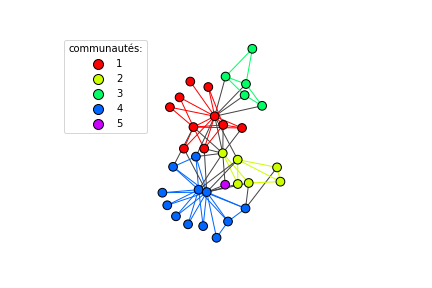
\includegraphics[scale=0.7]{images/G_zachary.png}
	\caption{Structures communautaires du graphe du club de karaté Zachary}
\end{figure}



Dans ce deuxième exemple, nous avons générer un graphe de manière aléatoire via la méthode $Erdos\_Renyi(n,m)$ où $n$ représente le nombre de sommets et $m$ le nombre d'arêtes du graphe.
Le modèle de Erdos-Rényi choisit un graphe uniformément au hasard parmi la collection de tous les graphes qui ont $n$ nœuds et $M$ arêtes.
Comme on peut le voir sur la figure 2, l'algorithme détecte qu'il y 9 communautés différentes dans le graphe. On remarque que ces différentes communautés sont mal séparées. On ne les distingue pas clairement.

\begin{figure}[H]
	\centering
	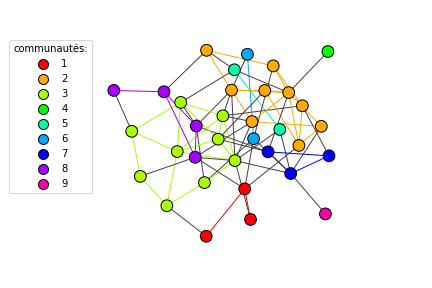
\includegraphics[scale=0.7]{images/random_network2.png}
	\caption{Structures communautaires d'un graphe généré aléatoirement}
\end{figure}


\section*{Annexes}
\addcontentsline{toc}{part}{Annexes}

Dans ces annexes vous trouverez une image présentant le fonctionnement de l'algorithme de Louvain ainsi que nos scripts qui ont été implémentés dans le but de faire de la détection de structures communautaires sur les deux graphes énoncés précédemment.

\begin{figure}[H]
	\centering
	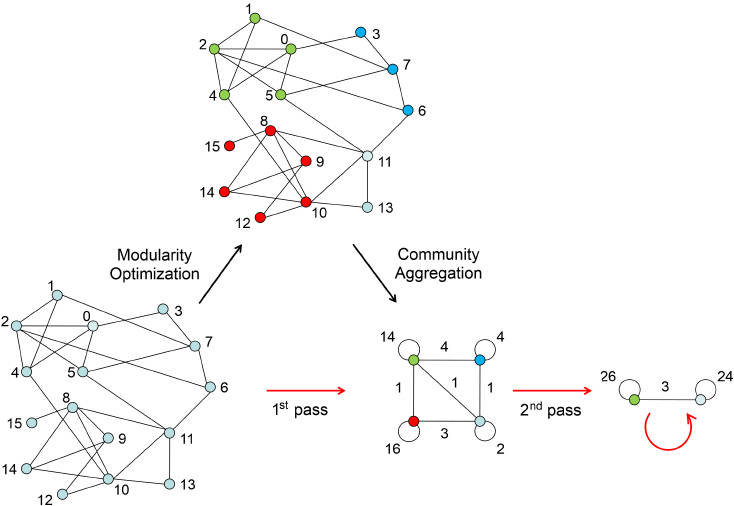
\includegraphics[scale=0.5]{images/Louvain.png}
	\caption{Application de l'algorithme de Louvain}
\end{figure}

\pagebreak

Ci dessous le script utilisé pour faire de la détection de communautés sur le graphe "Zachary"

\lstinputlisting[language=Python, firstline=9, lastline=61]{mon_code/zachary_karateClub.py}

\pagebreak

Ci dessous le script utilisé pour faire de la détection de communautés sur le graphe généré aléatoirement avec la méthode de $Erdos\_Renyi(n,m)$.

\lstinputlisting[language=Python, firstline=8, lastline=61]{mon_code/randomNetworkClustering.py}

\chapter*{Bibliographie}

\addcontentsline{toc}{part}{Bibliographie}

[1] WikiStat. An introduction to network inference and mining,\textit{Article}\newline
\url{http://www.nathalievialaneix.eu/doc/pdf/wikistat-network_compiled.pdf}\newline
\break
[2] PNAS. Modularity and community structure in networks (2015),\textit{Article}\newline
\url{https://www.pnas.org/doi/10.1073/pnas.0601602103#abstract} \newline
\break
[3] Wikipédia (2022). Méthode de Louvain, \textit{Article}\newline
\url{https://fr.wikipedia.org/wiki/Méthode_de_Louvain} \newline
\break
[4] igraph, \textit{Documentation}\newline
\url{https://igraph.org/python/versions/latest/}\newline
\break
[5] igraph, \textit{Documentation}\newline
\url{https://igraph.org/python/versions/latest/tutorials/visualize_communities/visualize_communities.html}
\break
[6] igraph, \textit{Tutoriel}\newline
\url{https://igraph.org/python/api/latest/igraph._igraph.GraphBase.html#Erdos_Renyi}

\end{document}